%!TEX root = ../thesis.tex
\chapter{User Needs}
\label{appendix:user-needs}
This section will define the user needs for the application.

\section{Personas}
%http://www.pewinternet.org/Reports/2010/Generations-2010.aspx 2010
%http://epp.eurostat.ec.europa.eu/portal/page/portal/statistics/search_database
%http://epp.eurostat.ec.europa.eu/tgm/table.do?tab=table&init=1&plugin=1&language=en&pcode=tin00097
%Individuals using the Internet for reading / downloading online newspapers / news magazines (tin00097)
\begin{figure}[h!tp]
\myfloatalign
\subfloat[Initial prototype layout with adjustable ratios between articles and a paged interface of each section.]{
  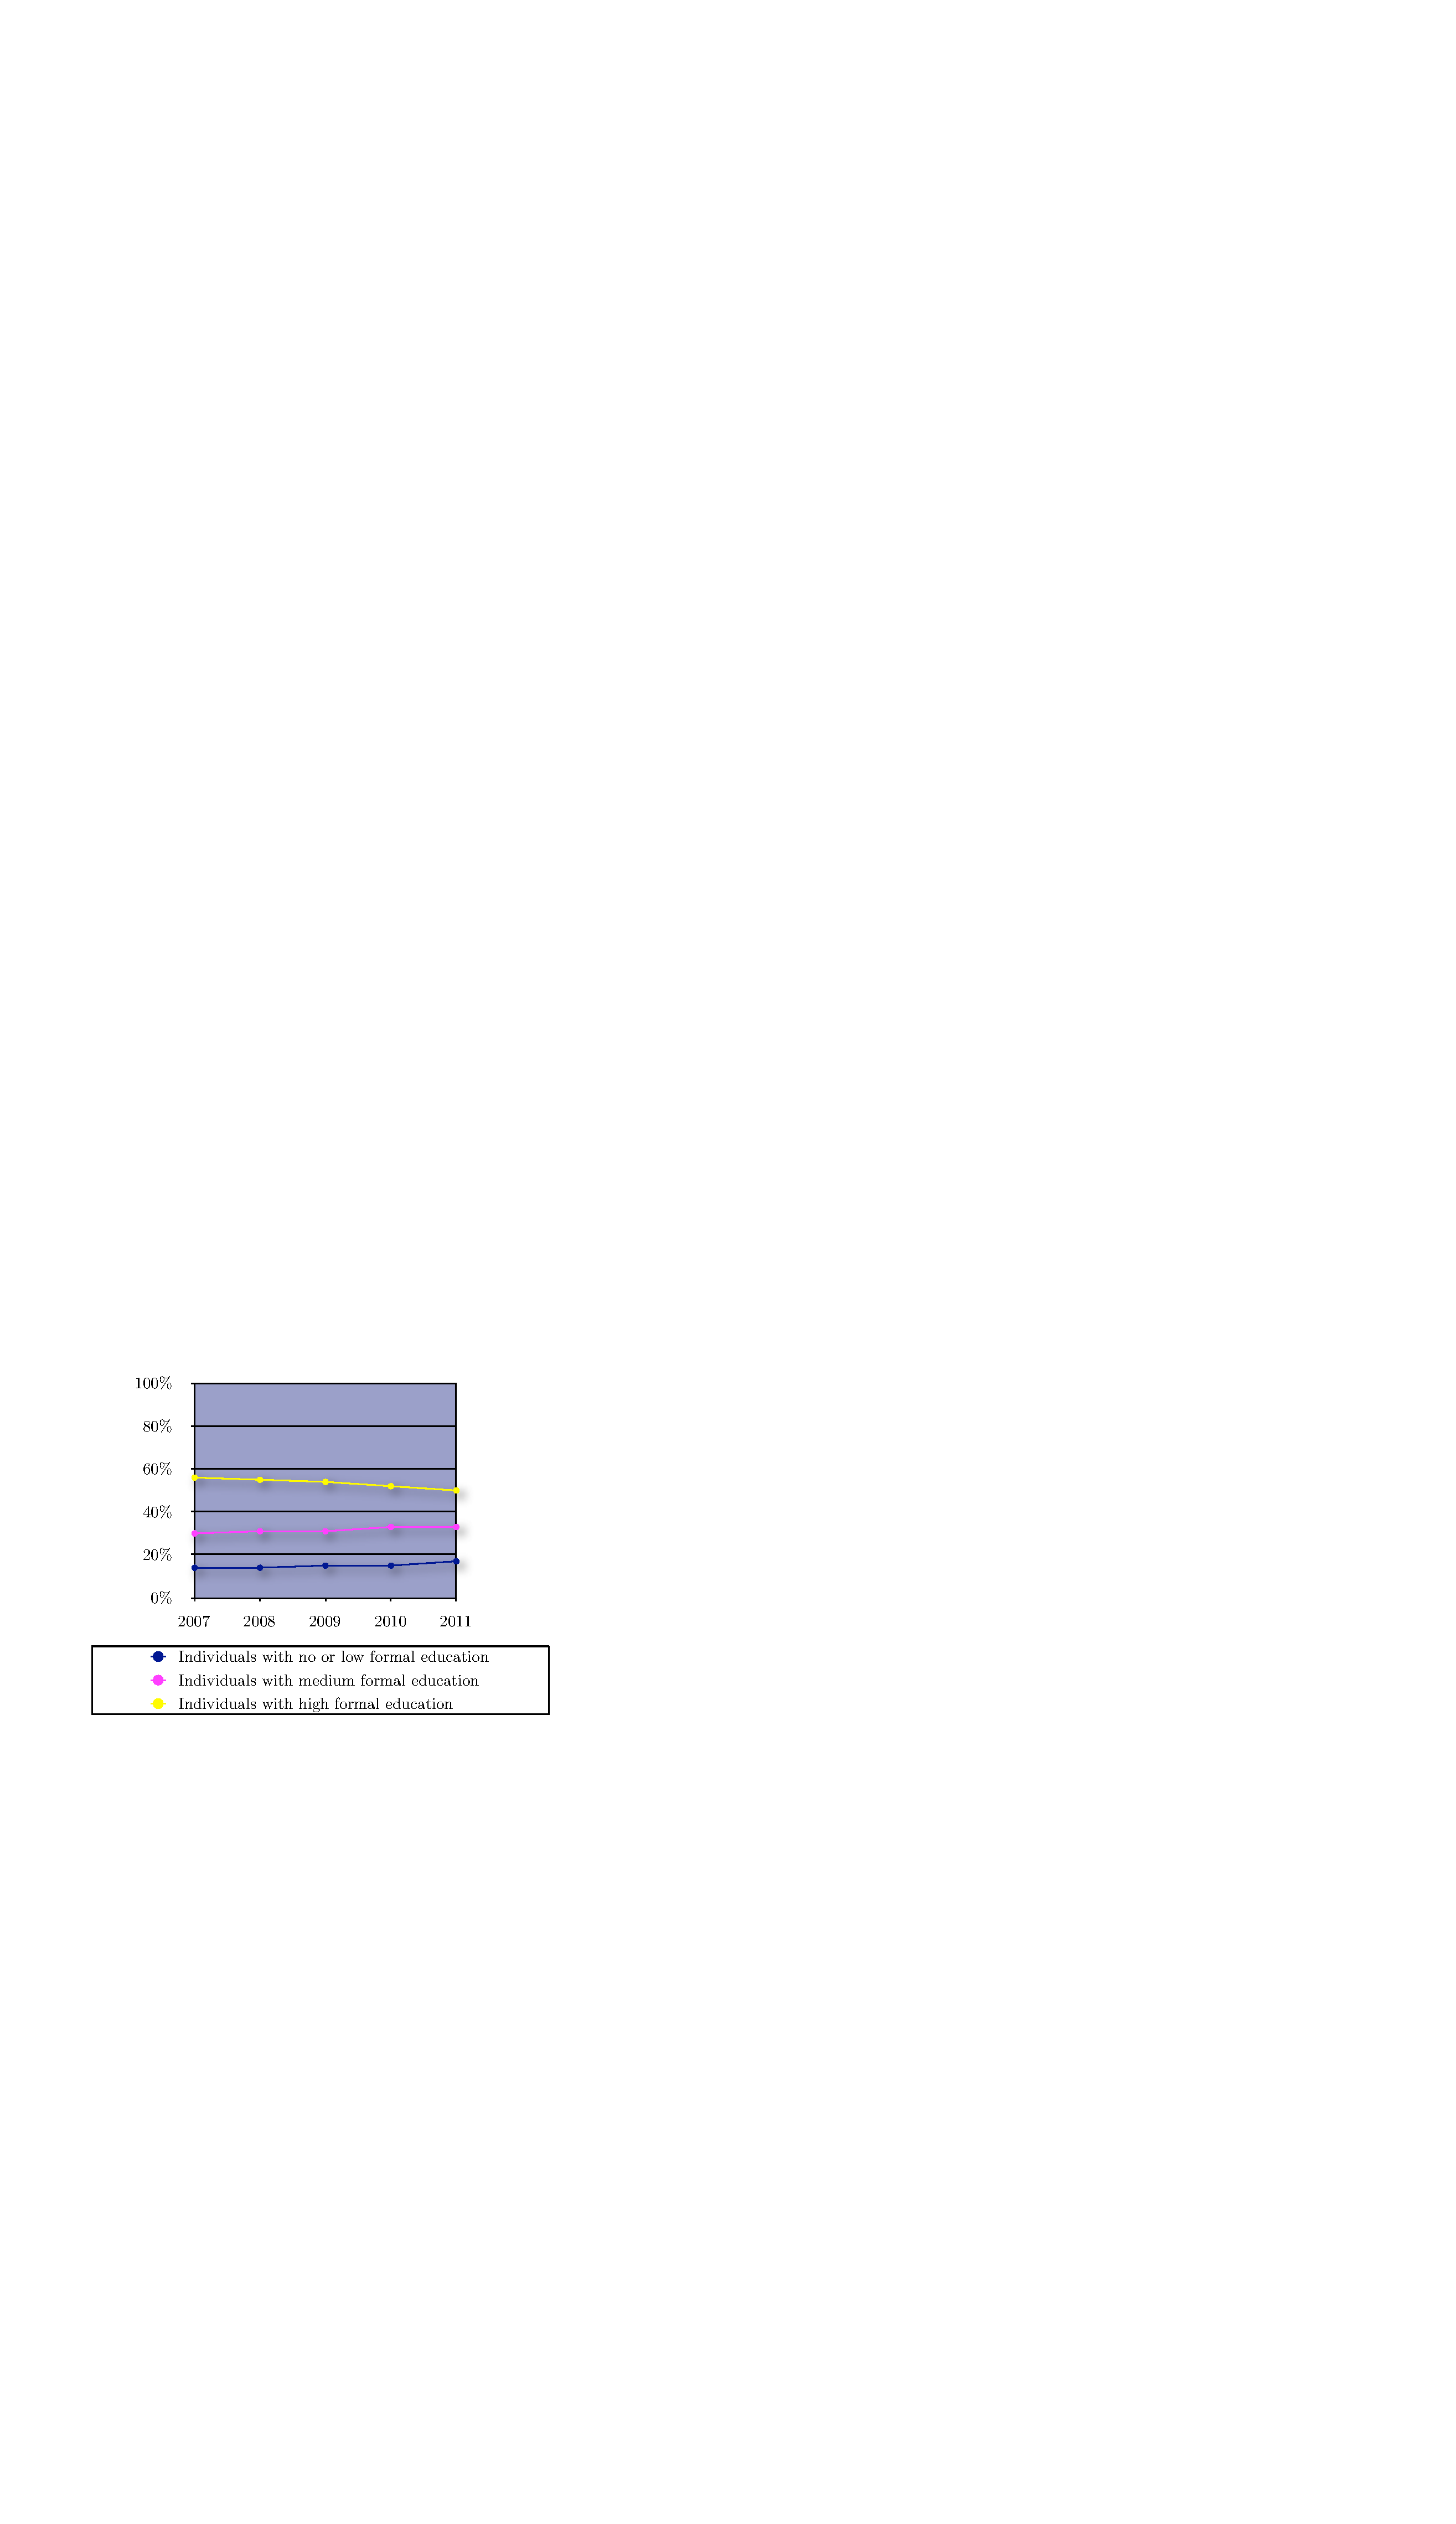
\includegraphics[width=.4\textwidth]{img/chart-educational.pdf}
  %\label{fig:prototype-iteration1}
} \qquad
\subfloat[Second iteration of the prototype with an ``endless'' layout. Sections are placed beneath each other.]{
  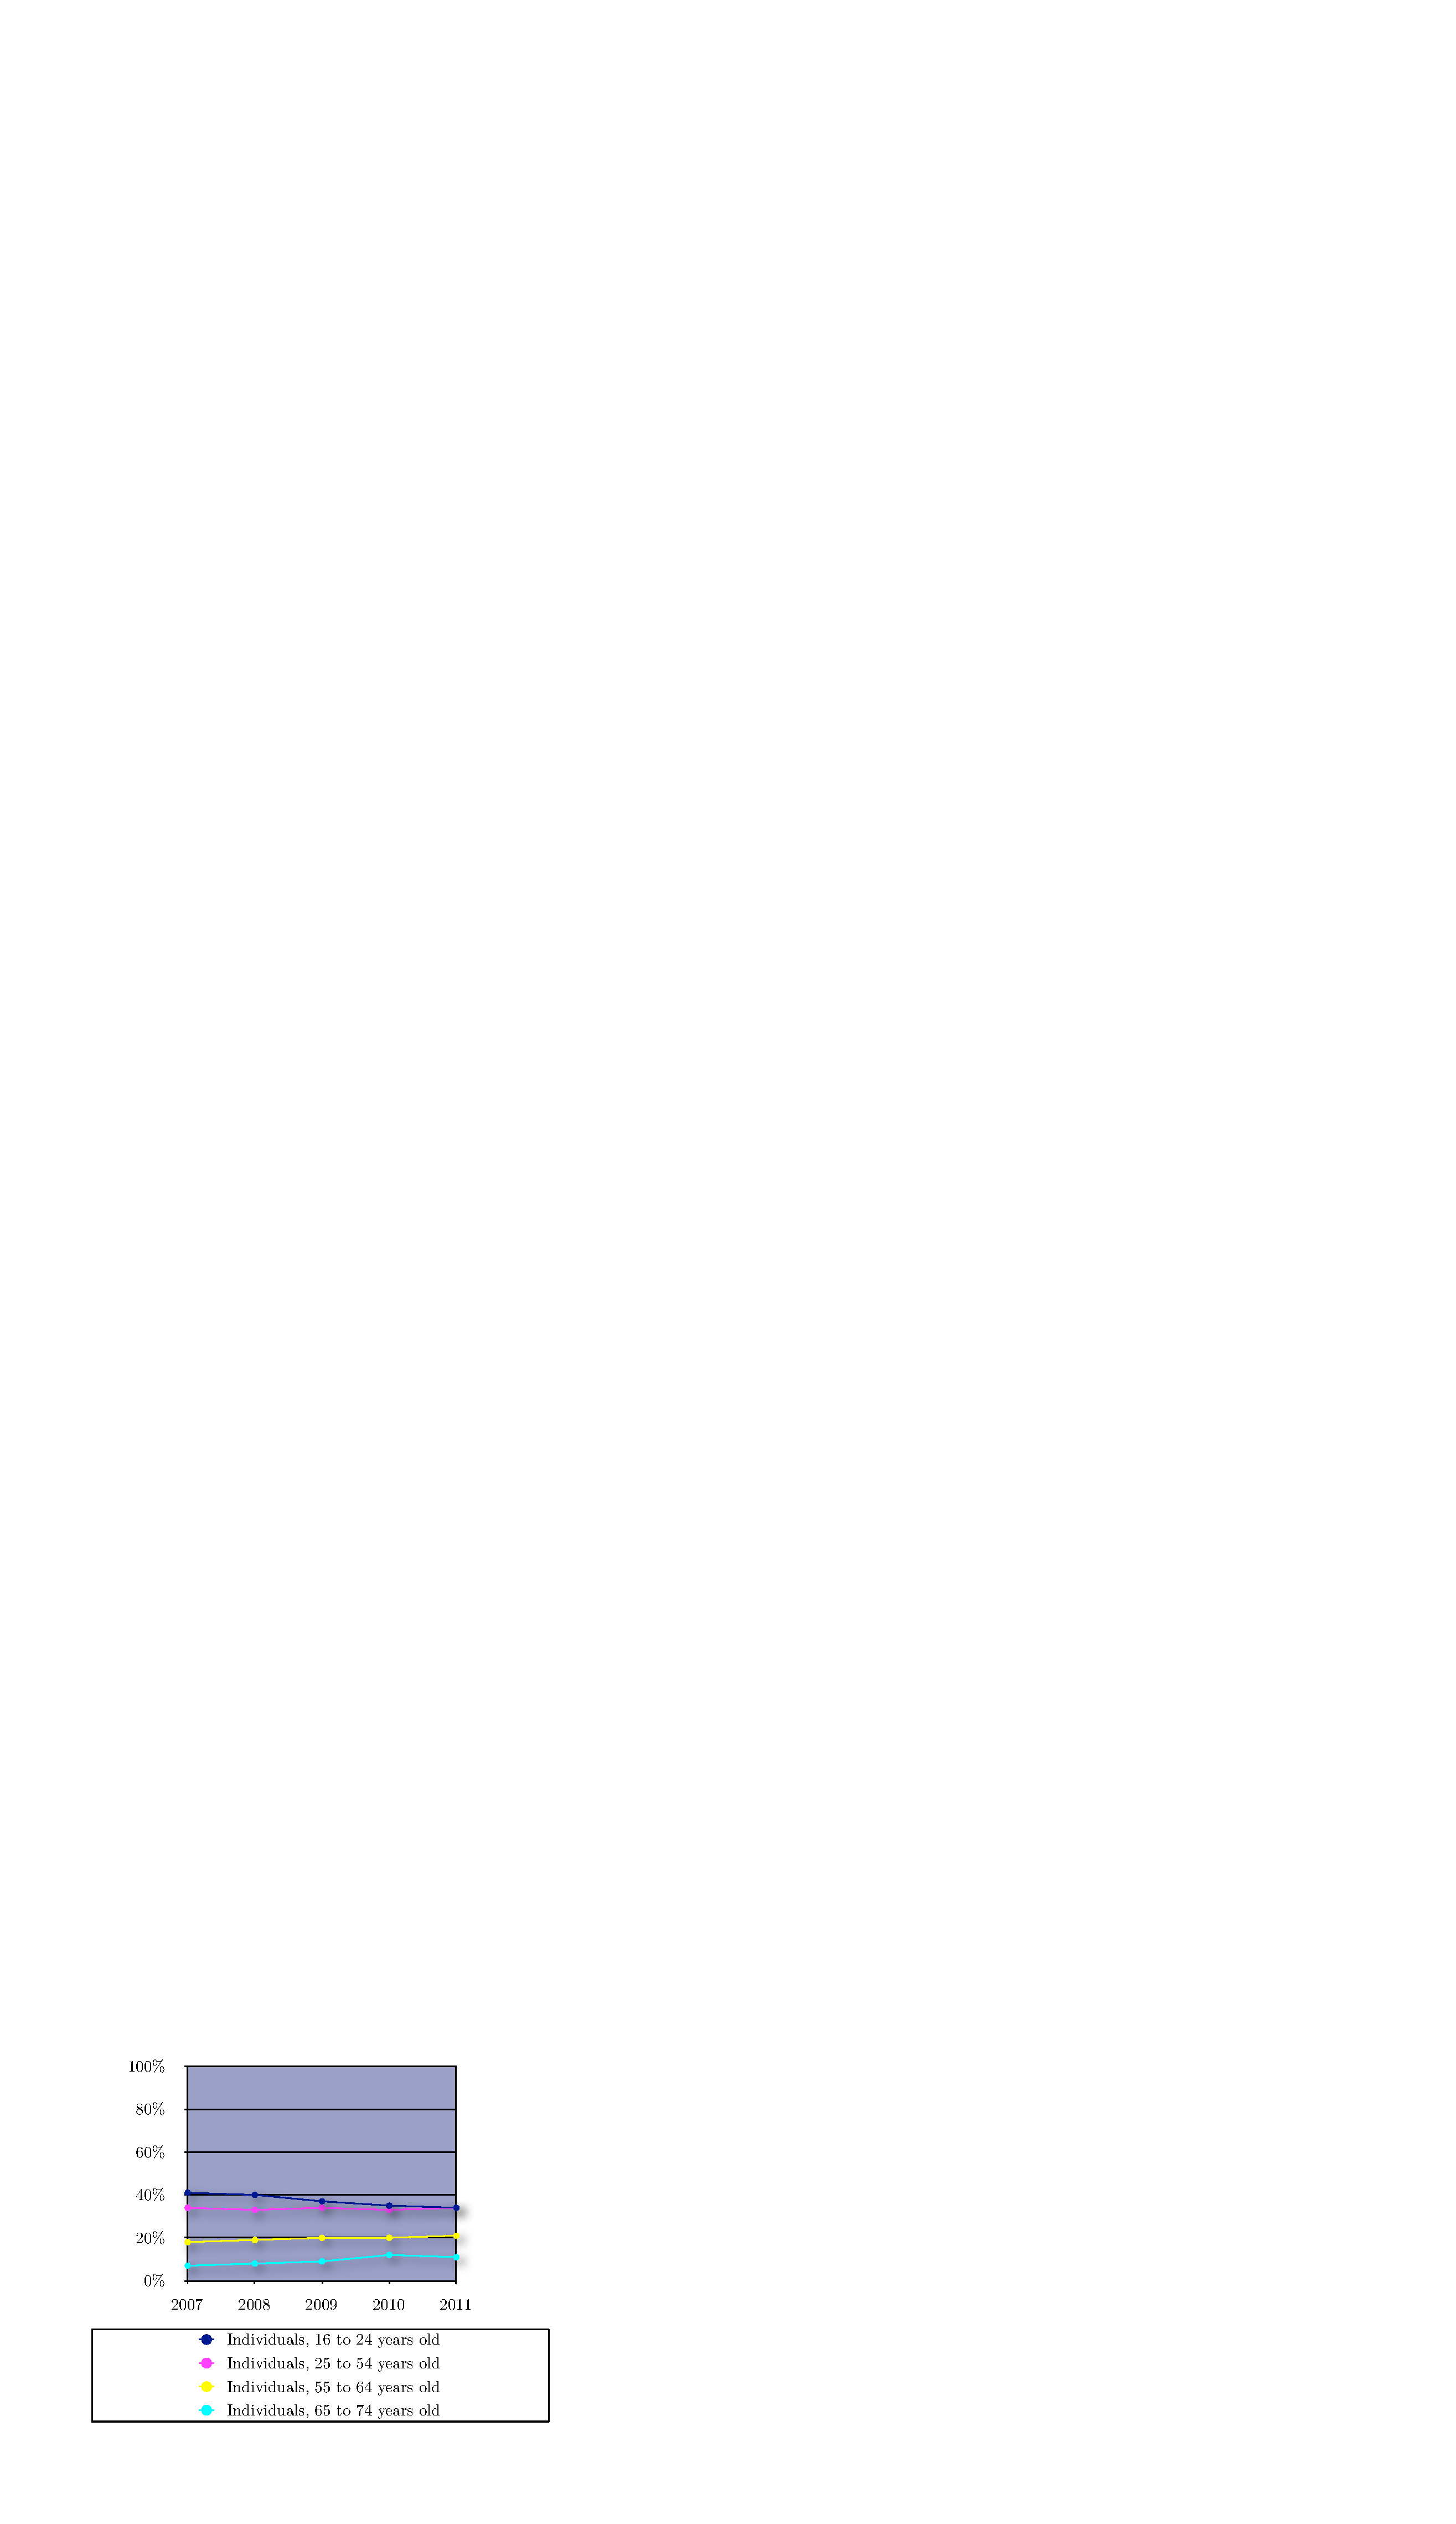
\includegraphics[width=.4\textwidth]{img/chart-individuals.pdf}
  %\label{fig:prototype-iteration2}
} \\
\subfloat[Third iteration of the prototype with a column-based and ``endless'' layout. Sections are placed beneath each other.]{
  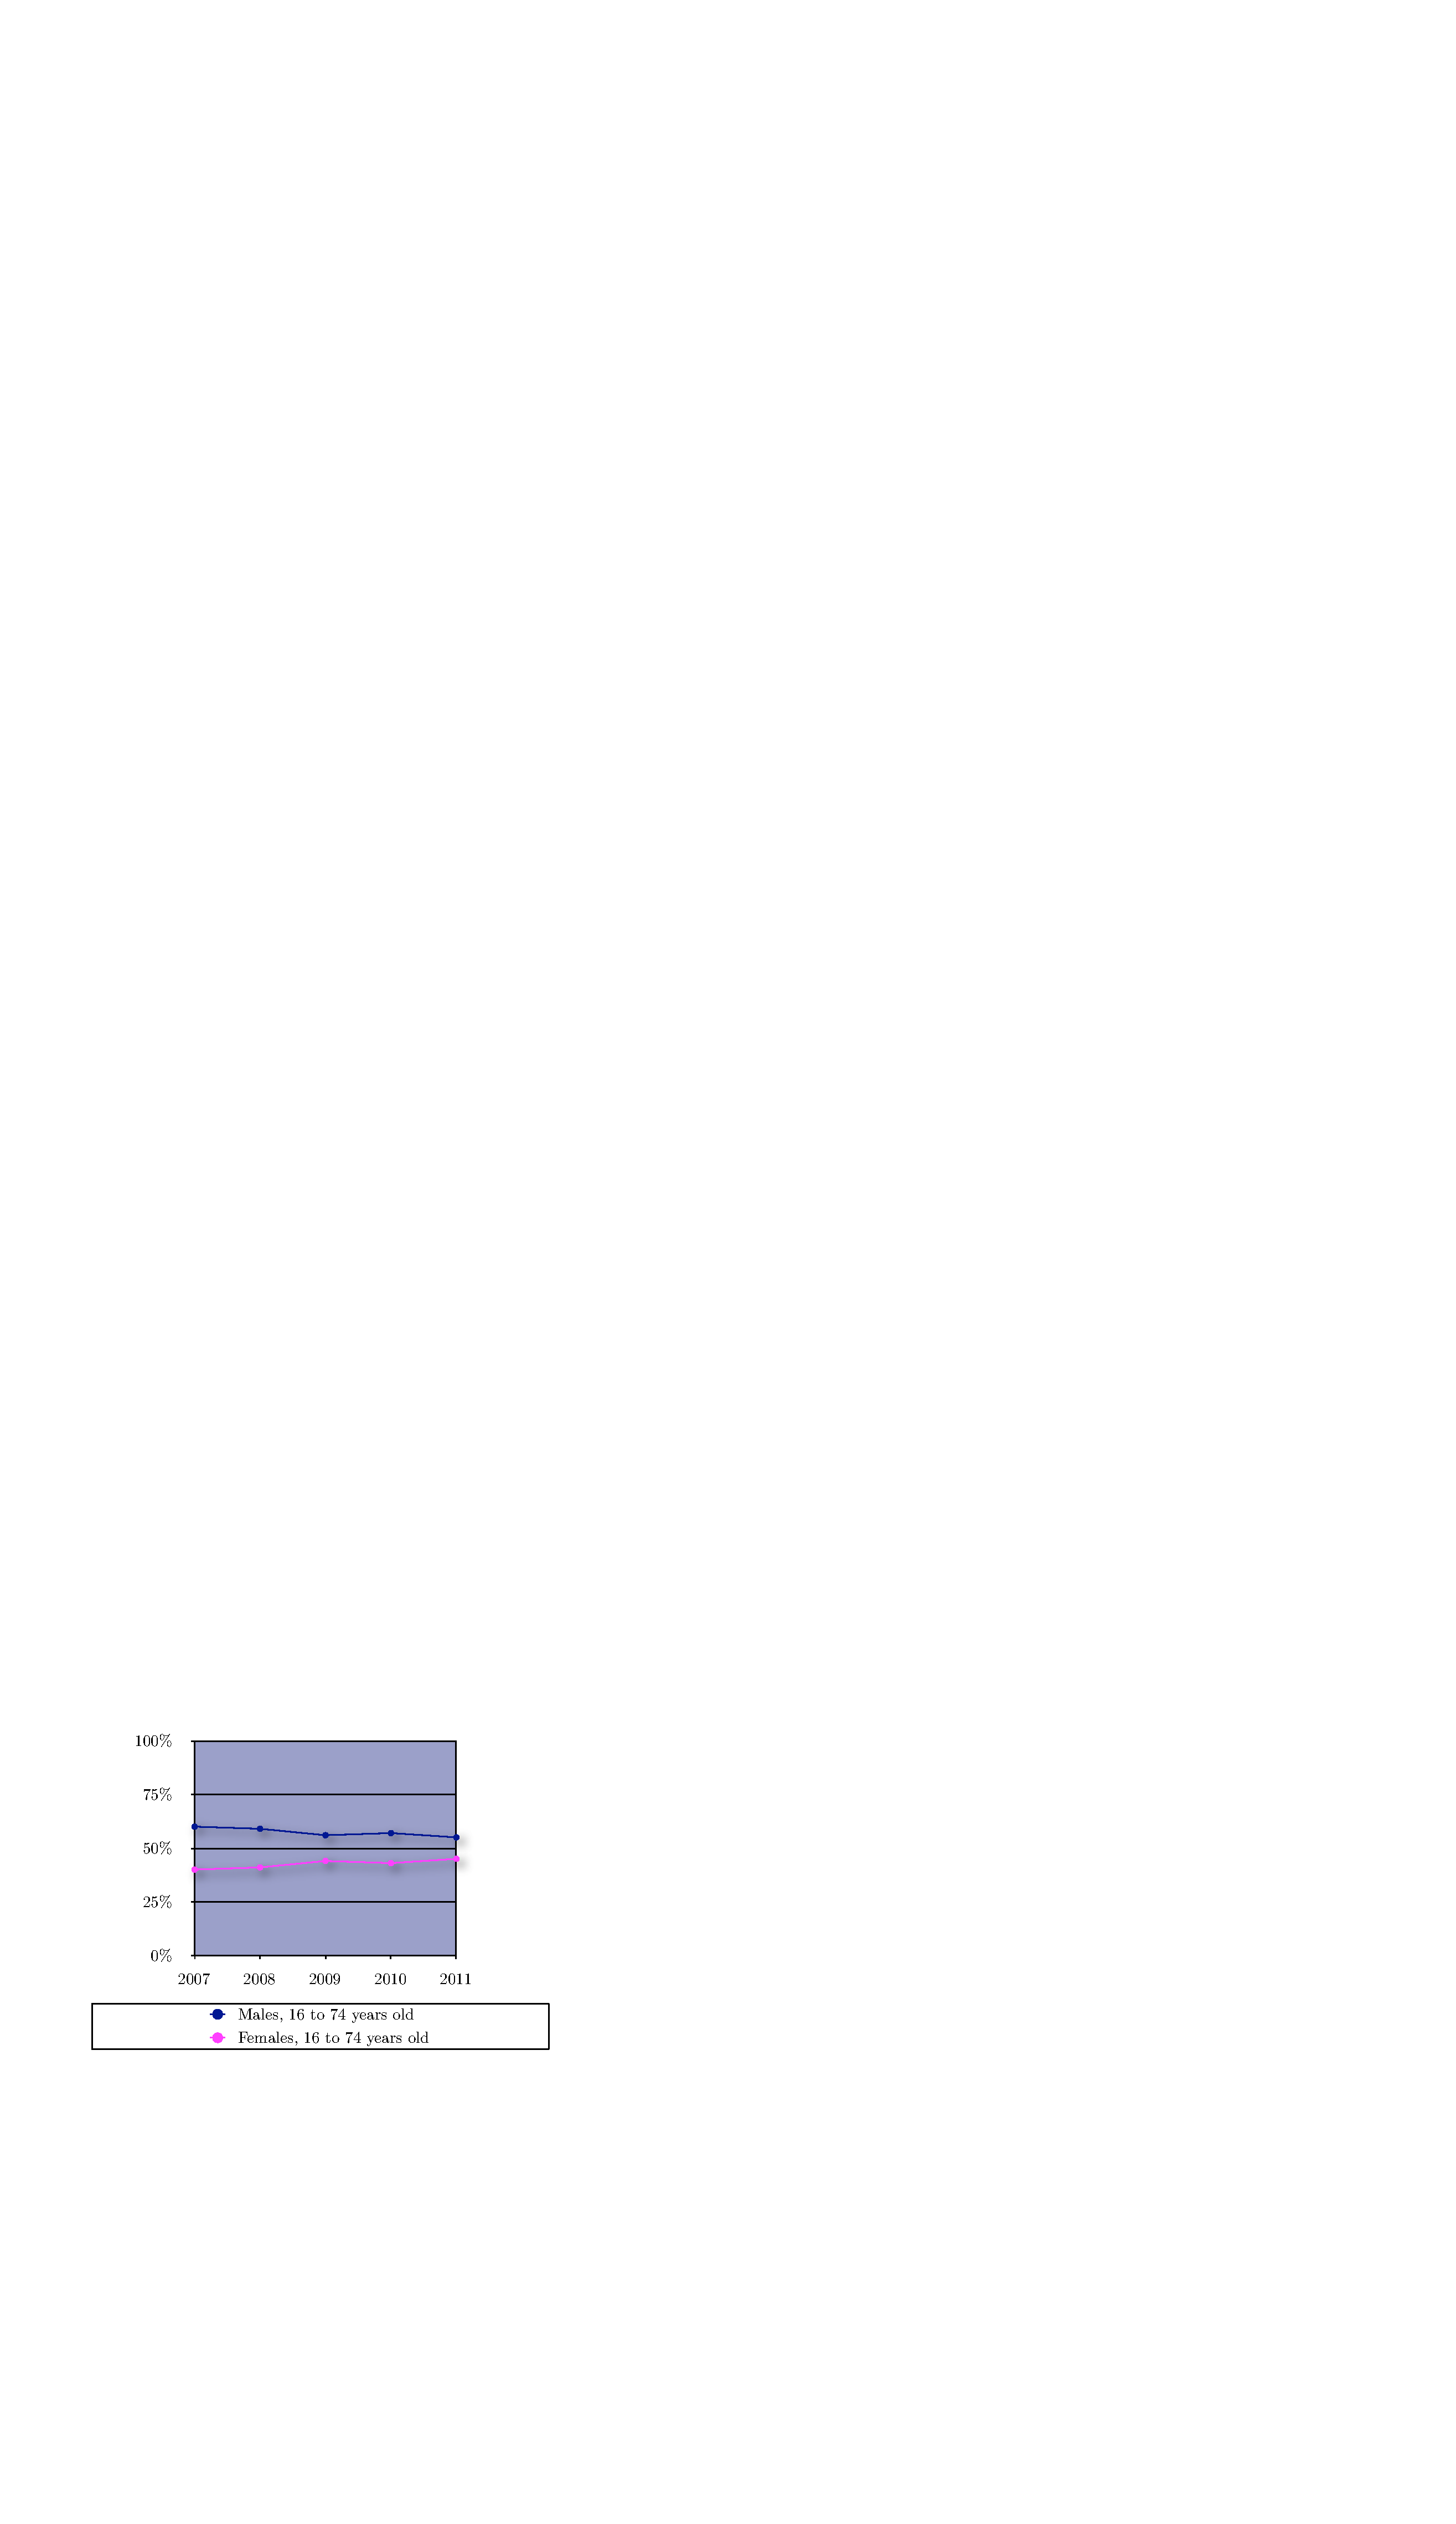
\includegraphics[width=.4\textwidth]{img/chart-males-females.pdf}
  %\label{fig:prototype-iteration3}
} \qquad
\subfloat[Third iteration of the prototype with a column-based and ``endless'' layout. Sections are placed beneath each other.]{
  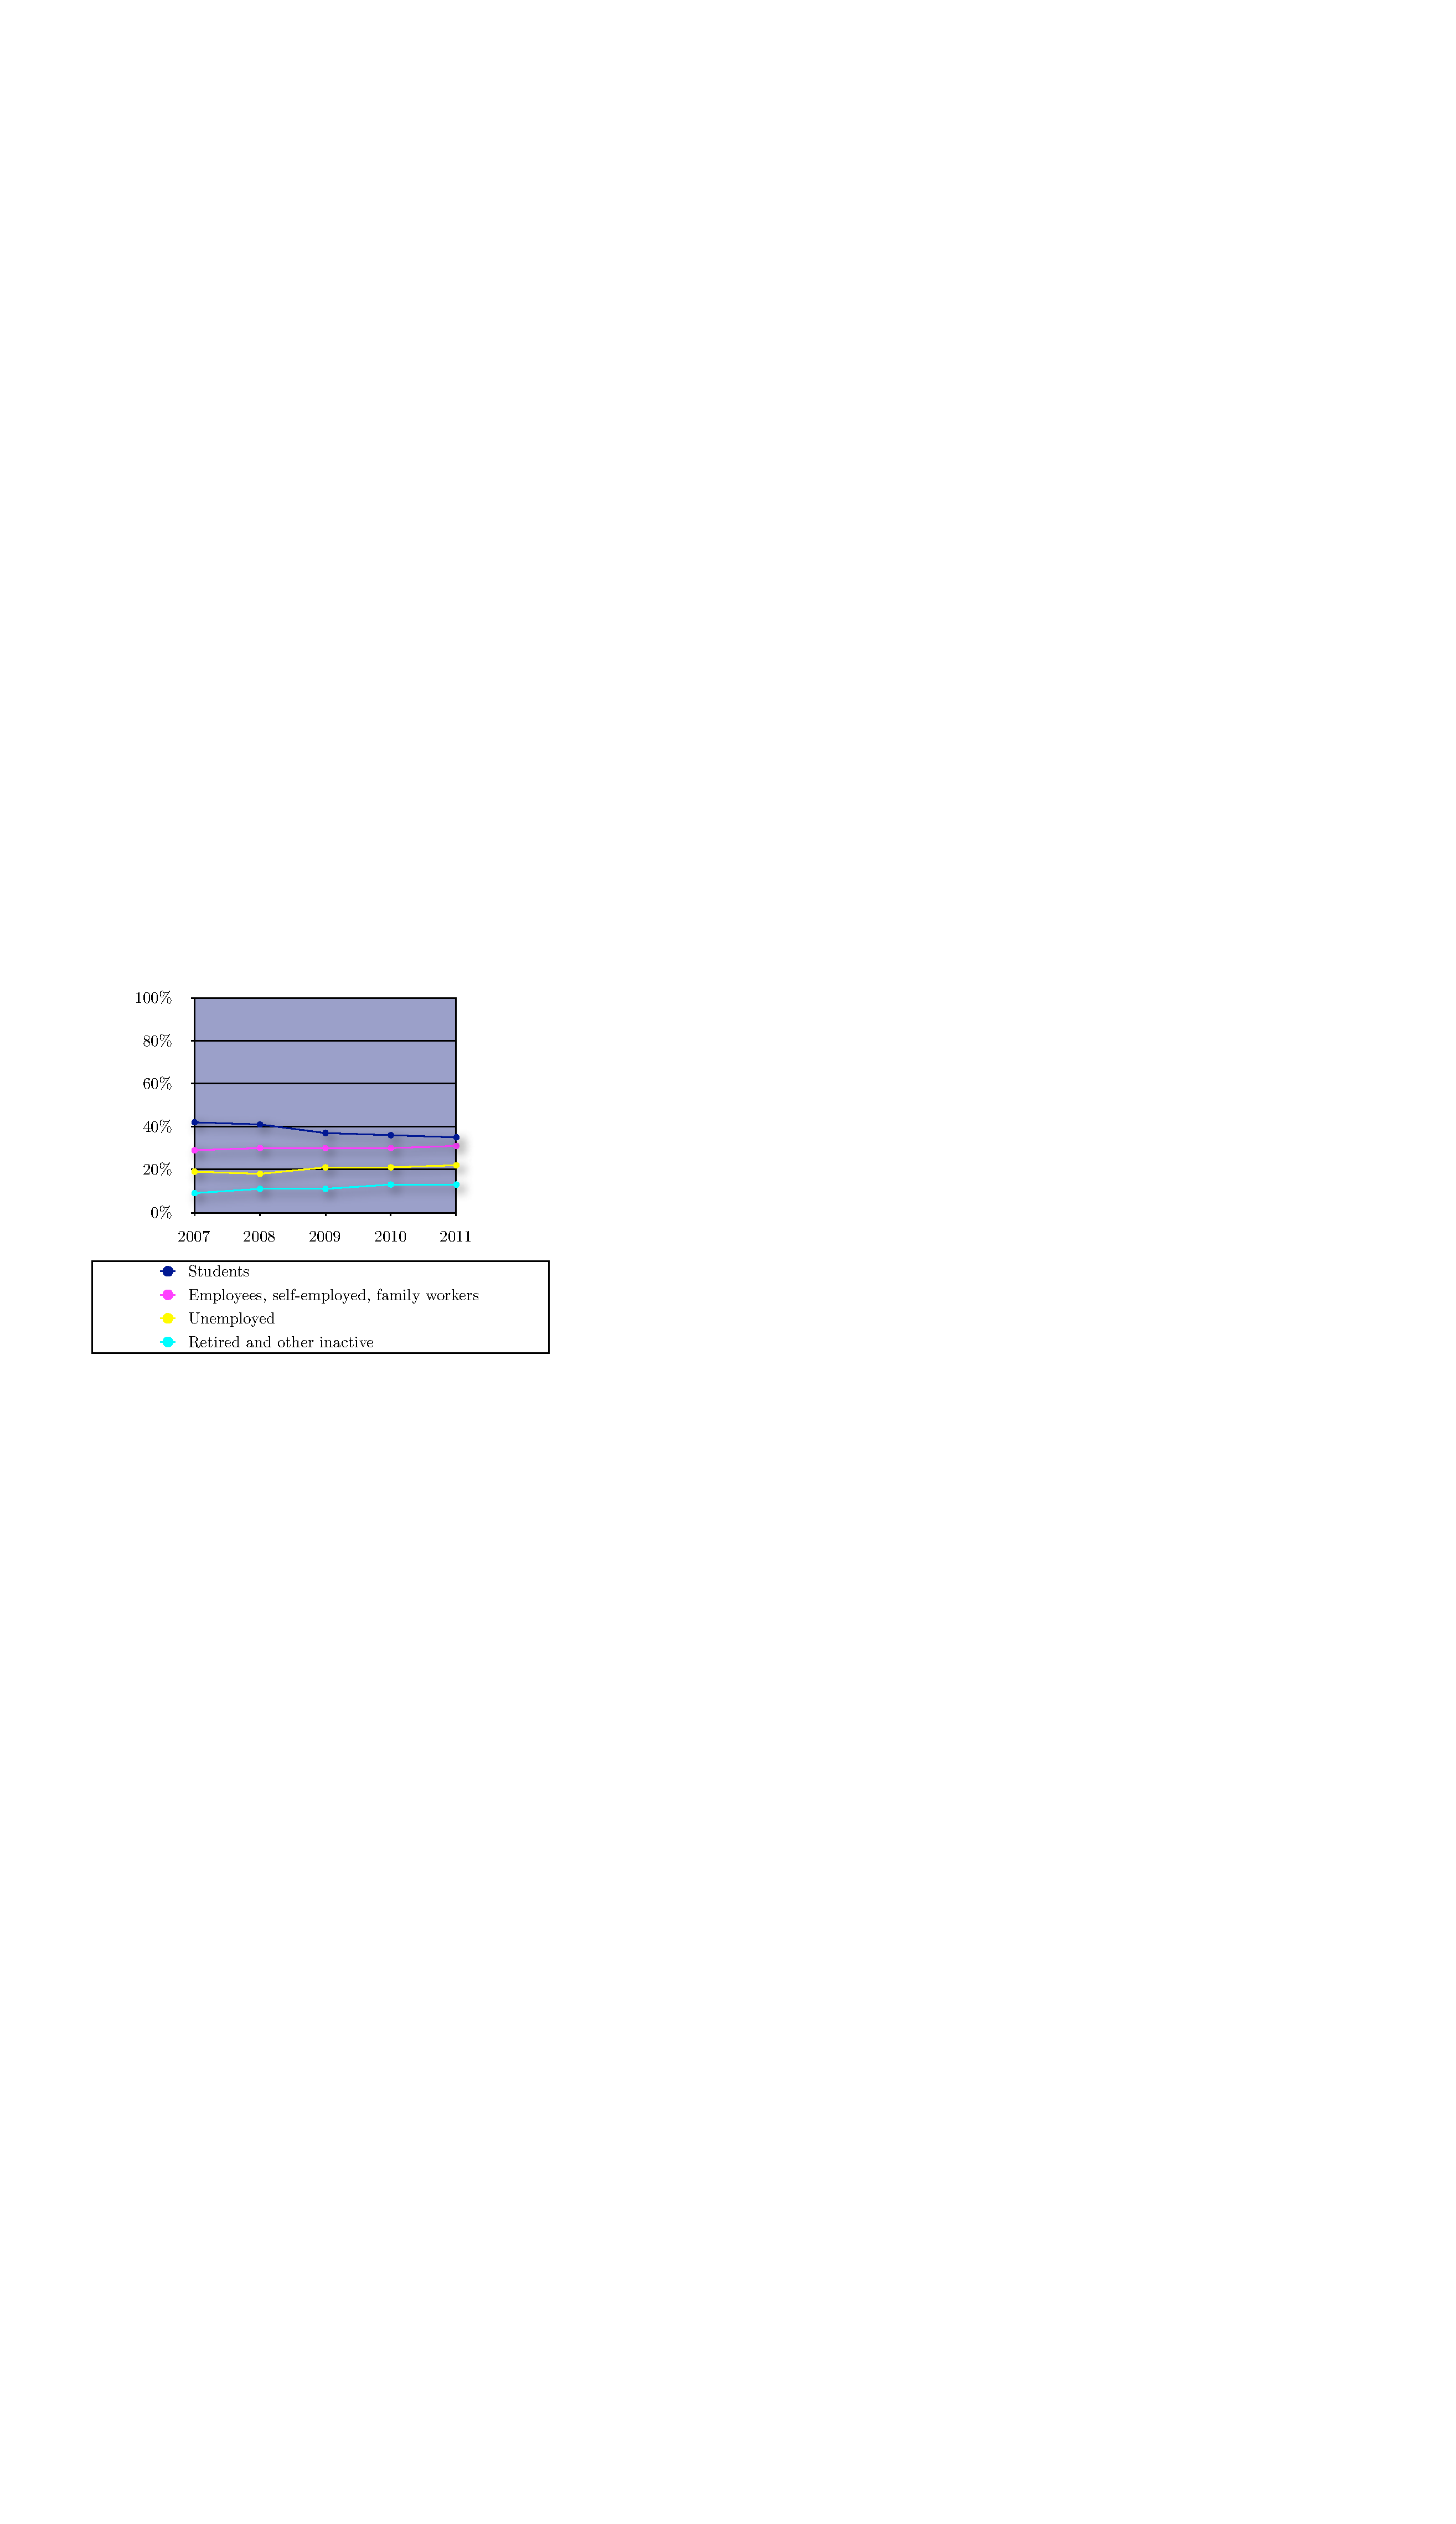
\includegraphics[width=.4\textwidth]{img/chart-occupation.pdf}
  %\label{fig:prototype-iteration4}
}
\caption{Eurostat: Individuals using the Internet for reading / downloading online newspapers / news magazines}
	\label{fig:charts-usergroups}
\end{figure}

In Figure~\ref{fig:charts-usergroups} is shown the basis for the division into the following user groups:

\begin{table}[h!tp]
\myfloatalign
	\marginnote{
		\begin{minipage}{\marginparwidth}
		%\vspace{-100pt}
		\caption{Eurostats distribution of individuals using the Internet for reading and downloading online newspapers and news magazines.}
		\label{fig:figurename}
		\end{minipage}
	}
	\begin{tabularx}{\textwidth}{p{.6\textwidth}|c}
		\toprule
		\textbf{Description} & \textbf{\%}\\
		\midrule
		\emph{student} & 35\\
		\midrule
		\emph{employees, self-employed, family workers} & 31\\
		\midrule
		unemployed & 22\\
		\midrule
		retired or other inactive & 13\\
		\bottomrule

		\textbf{Description} & \textbf{\%}\\
		\midrule
		\emph{high formal education} & 50\\
		\midrule
		medium formal education & 33\\
		\midrule
		no or low formal education & 17\\
		\bottomrule

		\textbf{Description} & \textbf{\%}\\
		\midrule
		\emph{male} & 55\\
		\midrule
		female & 45\\
		\bottomrule

		\textbf{Description} & \textbf{\%}\\
		\midrule
		\emph{16-24} of age & 34\\
		\midrule
		\emph{25-54} of age & 34\\
		\midrule
		55-64 of age & 21\\
		\midrule
		65-74 of age & 11\\
		\midrule
	\end{tabularx}
\end{table}

The user groups provide the basis for the following personas.

\subsection{Thomas: student medium formal education male of age 21}
Thomas is 21 and a student at the Technical University of Denmark to be a bachelor of engineering in software. He is very interested in soccer and is therefore always updated on sports news. He reads about it online, newspapers and talks about it with friends. With big events he even likes to post it on Facebook. As a soon-to-be software engineer he has a natural thirst for news about technology, and he mainly reads these at home at the dormitory.
wired.com, newz.dk, engadget.com, facebook.com
computer, Samsung Galaxy Tab

\subsection{Laura: employed high formal education female of age 39}
Laura is 39 and is employed as a key account manager. She likes to be updated on strategies and economical status of rivalling companies. She is also very interested in politics and likes to discuss this subject with her friends. She reads economical news and likes to be updated on the run.
b.dk, borsen.dk, twitter.com
iPhone, iPad

\subsection{Marie: unemployed no or low formal education female of age 61}
Marie is 61 and a currently unemployed housekeeper. She spends her day looking for a job and taking care of her pet cat until her husband comes home. She mostly looks for the gossip sections or news about crime or big disasters. She also spends some time reading through the travelling guides as she dreams of going away with her husband.
ekstrabladet.dk, bt.dk, nyhederne.tv2.dk
computer, Lenovo IdeaPad A1

\subsection{Carl: retired or other inactive high formal education male of age 69}
Carl is a retired professor in psychology. He likes to discuss human behaviour and relation with his acquaintances and is very interested in cultural events. Therefore he often seeks the cultural sections and discussion fora to see what is going on. 
politiken.dk, aok.dk, dr.dk
computer, iPad

\section{Scenarios}
\subsection{Thomas}
Thomas comes home after a day at the study, picks up his tablet computer and opens Editor from the desktop. Editor opens and shows him the front page where all the headlines stories are displayed. The main story is about a new version of the Android OS that has been released today and presses it to read more. The story opens in a full window display with quality images to match the articles. He reads the first section and feels satisfied with the amount of information, but wants to share the information on Facebook, so he clicks share button and writes a comment and posts it on his Facebook wall. He closes the article and returns to the front page. He sees a top story below the main story about Mr. Mærsk Mc-Kinney Møller who has died. It is not a story that falls into his key interests, but as the news is big he is satisfied that he got informed about it. Thomas feels like reading more about technology so he opens the menu and chooses the ``Tech'' section he has installed in the application. The section opens with a head line and a page number to let him know where in his paper he has navigated to and finds an article about a new multicore CPU technology. He has never been interested in CPU technology before, but finds this technology interesting after reading about it, so he opens the application settings and types in keywords about the technology under his ``Tech'' section to keep him updated about it. He also adjusts the ratio between general and personal news, to be less personal as he feels like he needs to broaden his horizon a bit with respect to news. He closes the settings menu and Editor immediately starts updating the articles. Some new articles about CPU technology has been included amongst the articles in the ``Tech'' section after paging through the section and reading some of the most interesting articles he closes the application.

It could be nice if the key words of a story could be or is already highlighted, so he can click it and add it to his positive or negative list.

\subsection{Laura}
Laura is on the train on her way to a business meeting this morning and pulls out her tablet and sees she has one notification from Editor. She opens Editor to get updated on todays news. The front page is displayed and there are headlines from different top articles and a notification is shown in the corner. She presses the notification and the pages turns to show her the article, which opens in full screen. After reading it she wants to see todays headlines, so she presses the back button to return to the paper and presses the return to front page button and the paper turns pages to reach the front page. She scans the page to see if there is any big news about her rivalling companies. There is no breaking news, so she just turns the page to browse the content of todays paper. As she browses the ``Politics'' section of her paper she finds an article about the Prime Minister introducing a new bill about a toll ring around the capitol city. She chooses the article and it is shown in full screen. As she reaches the bottom of the article she sees the comments about it where her friends and most others are against it. She decides to join the discussion and posts a comment on the article wall. She also sees one of her friends has not commented on the article wall and decides to share the article with her as she thinks she would agree with her opinion. She presses the share button and chooses the Editor logo. A list of her friends is shown, some of them who has already read the article is greyed out, but the one she was looking for is not. So she chooses her and a notification is sent to her.

\subsection{Marie}
It is morning and Marie wants to check the news with her coffee in the couch, so she opens Editor from her tablet to get updated. The front page is displayed with a collection of stories as highlights of the content of the paper. It mainly contains stories about celebrities and a big disaster that has happened in japan, but there is also a story about a big political change, that she does not find interesting. So she goes to the settings menu and types in ``politics'' to add to her negative list. She also adjusts the personal/general news ratio to contain only personal news as she wants only news that is directed to her. She returns to the front page which is now free of political stories. Her newspaper contains many images and videos as she has set her graphical/textual content ratio more towards graphical content.

\subsection{Carl}
Sunday morning Carl wakes up, puts over the kettle to make a cup of coffee. While he waits for the water to boil he picks up his iPad and opens Editor to check the news. The front page opens with headlines from the different sections. There is a review article about a new show in the theatre. Carl presses the article and the system turns pages to the ``Cultural'' section of his newspaper and opens the article in full screen. Because the show gets good ratings he decides to order some tickets to him and his wife, which he does using the devices browser. After this he reopens Editor which opens in a display of the same article, as he left it. Carl pours his coffee and turn to the back page with the some crossword puzzles and some cartoons. He presses a puzzle that looks funny and it is displayed in a full page, where he can solve it. When he is done he returns to the page and chooses his regular cartoon to read.

\section{Business Case}
\subsection{Need}
User value: personal quality and up-to-date stories enriched with quality images. This means that content providers should be chosen/verified. Same navigation as actual newspapers, but faster and with endless more content. Instantly up-to-date. Adaptive layout. Adjustable to individual user.

\subsection{Approach}
Personalised content in an editorial mix.

Constraint Programming: fast computation - good for optimal solutions, describes the generic solution in stead of how to solve or find it, easy to tailor the problem definition of the solution and adjust it and even let users make the adjustments - transparency.

Content providers can get to know their readers preferences better and improve the provided content.

\subsection{Benefit Per Cost}
Revenue flow: Content providers are paid. Income from advertisers (scattered \cite[p. 6-7]{kristin_fredrik.pdf}) and users. Income from selling user behaviour patterns and precise targeted commercials.

\subsection{Competition}
FlipBoard, Wired magazine, Zite and app with actual editors affiliated.

\section{Requirements}
The above scenarios, user needs and business case led to the following requirements.

\subsection{Non-functional Requirements}
\begin{itemize}
	\item ``the clear overview of content, including a beginning and an end, the ease of use, typography and design'' \cite[p. 7]{FULLTEXT01.pdf}
	\item both general and personal news (collaborate filtering solves that some news are not received, but are universally interesting \cite{fulltext.pdf})
	\item familiarity in design from printed paper \cite[p. 7]{FULLTEXT01.pdf}
	\item Design and layout from printed newspaper \cite{hcii2005_1004.pdf}
	\item both images and videos - test
	\item a good ratio of graphical and textual - test
	\item front page should give a good overview of the content - test
	\item ``news valuation, e.g. positioning of lead story'' \cite[p. 7]{FULLTEXT01.pdf}
	\item  mobility \cite[p. 7]{FULLTEXT01.pdf}
	\item  continuous updates \cite[p. 7]{FULLTEXT01.pdf}
	\item ``easy and intuitive navigation'' \cite[p. 7]{FULLTEXT01.pdf}
	\item add video and sound \cite[p. 7]{FULLTEXT01.pdf}
	\item incorporate social community and social networks
\end{itemize}

\subsection{Functional Requirements}
\subsubsection{Calculations on number of columns}
\label{sec:column_calc}
iPad screen size:

$197 \times 148mm$ or $1024 \times 768px$

International Herald Tribue (the global edition of the new york times): $\frac{398mm}{6} = 66.333333333mm$

Børsen (uses both 5 and 6 columns): $\frac{285mm}{5} = 57mm$ and $\frac{285mm}{6} = 47.5mm$

Information (5 columns 4 on the back): $\frac{285mm}{5} = 57mm$ (back $\frac{285mm}{4} = 71.25mm$)

Guardian (5 columns): $\frac{314mm}{5} = 62.8mm$

Politiken (6 columns): $\frac{392mm}{6} = 65.33mm$

Berlingske (4 columns): $\frac{285mm}{4} = 71.25mm$

Average on the most regular columns:

$\frac{66.3+57+57+62.8+65.3+71.3}{6} = 63.283333333mm$, i.e.\ $3.11$ columns in landscape and $2.34$ in portrait.

(Average on every column width:

$\frac{66.3+57+47.5+57+71.25+62.8+65.3+71.3}{8} = 62.30625mm$, i.e.\ $3.16$ columns in landscape and $2.38$ in portraint.)

$1200px$ screen:

$\frac{1200 \cdot \frac{197}{1024}}{63.28} = 3.65$ columns, where 197/1024 is $px$ to $mm$ ratio and 63.28 is the thinnest column width

column size in px:

$63.28 \cdot \frac{1024}{197} = 329px$

$62.31 \cdot \frac{1024}{197} = 324px$

average $= 326px$

\begin{itemize}
	\item 2 columns in portrait and 3 in landscape
	\item ``open, turn pages, chose article, read and return'' \cite[p. 6]{FULLTEXT01.pdf}
	\item section headlines \cite[p. 6-7]{kristin_fredrik.pdf}
	\item article headlines
	\item article summaries / extracts \cite{fulltext.pdf}
	\item menu w. section headlines \cite[p. 8]{kristin_fredrik.pdf}
	\item page numbers \cite[p. 6-7]{kristin_fredrik.pdf}
	\item press ``like'' or key word based user profile (mark self or highlighted? right click to add): positive + negative list (keywords+categories \cite{10-1-1-19-5583}, \cite{fulltext.pdf} and \cite{gervasum2001ws.pdf})
	\item full screen display of article
	\item organise into personalised sections
	\item opens in front page view (summery of newspaper 8 articles) \cite[p. 8]{kristin_fredrik.pdf}
	\item adjust variables
	\item share directly (grey out the ones who have read it)
	\item comment
	\item see friends comments
	\item ``The presentation schema -- headline, abstract, and text, together with a relevance value with respect to the user profile -- rates the highest in terms of user satisfaction, and yet it is not the most frequent.'' \cite{Sections-categories-and-keywords-as-interest-specification-tools-for-personalised-news-services.pdf}
	\item  ability to search \cite[p. 7]{FULLTEXT01.pdf}
	\item Landscape + portrait \cite[p. 6-7]{kristin_fredrik.pdf}
	\item touch screen interaction \cite[p. 6-7]{kristin_fredrik.pdf}
	\item Functionality from online newspaper \cite{hcii2005_1004.pdf}
	\item Name of columnist \cite[p. 4]{gervasum2001ws.pdf}
	\item Transparency of implicit relevance feedback (see/modify current weights of categories) \cite[p. 7]{gervasum2001ws.pdf}
	\item dynamic short-term + static long-term user profile \cite{10-1-1-19-5583}, \cite{fulltext.pdf} and \cite{gervasum2001ws.pdf}
	\item relevance feedback \cite{10-1-1-19-5583}, \cite{fulltext.pdf} and \cite{gervasum2001ws.pdf}
\end{itemize}

\section{Test Results}
\label{sec:test_results}
This section sums up the test results in an unordered list.
\begin{itemize}
 \item Touch friendly interaction
 \item Tools for changing the layout, like changing the font size and colour scheme
 \item The front page should give an overview
 \item View whole menu all the time
 \item Give suggestions to similar articles, i.e.\ more on this story, subject and topic
 \item List overview of headlines in top of sections
 \item Search within relevant articles. Search bar should be visible at all times.
 \item Indication of similarity on articles
 \item Archive possibility
 \item User feedback notated with ``relevant'' and ``irrelevant''
 \item White space besides articles is not a problem
 \item General layout corrections
 \item Better visual division between articles
 \item More and larger images
 \item No need for general news, personalised news is enough
 \item Choose categories with topics to get started
 \item Ability to choose period show articles from
 \item Ability to choose when the newspaper should be generated, e.g.\ on Fridays to be read in the weekend
 \item Dividing columns into screens
 \item Social community implementation
 \item Visualisation of user behaviour
 \item Possibility to use it for research
 \item Get articles from magazine and newspaper subscriptions, e.g. by adding them to a specific section
 \item It has solved the problems that \url{http://nyhederne.tv2.dk/}\sidenote[1]{The website of a Danish news channel.} has, i.e.\ confusing layout, no overview and hard to navigate
\end{itemize}